\pdfminorversion=7
\documentclass[convert={density=600,outext=.png},multi=tikzpicture,tikz]{standalone}
\usetikzlibrary{arrows, calc, fit, hobby, positioning}
\pdfsuppresswarningpagegroup=1
\graphicspath{{../system}}
\usepackage{xcolor}
\AtBeginDocument{\pagecolor{black}\color{white}}
\begin{document}
\foreach \stage in {1,...,3}{\begin{tikzpicture}[>=stealth']
 \tikzset{
  arrownode/.style={fill=black, font=\tiny, inner sep=.5pt},
 }
 \path[use as bounding box] (5.5, 1.5) rectangle ++(5.85, -4.9);

 \node [draw, fill=black] (CPG_r) at (6.5, -2.5) {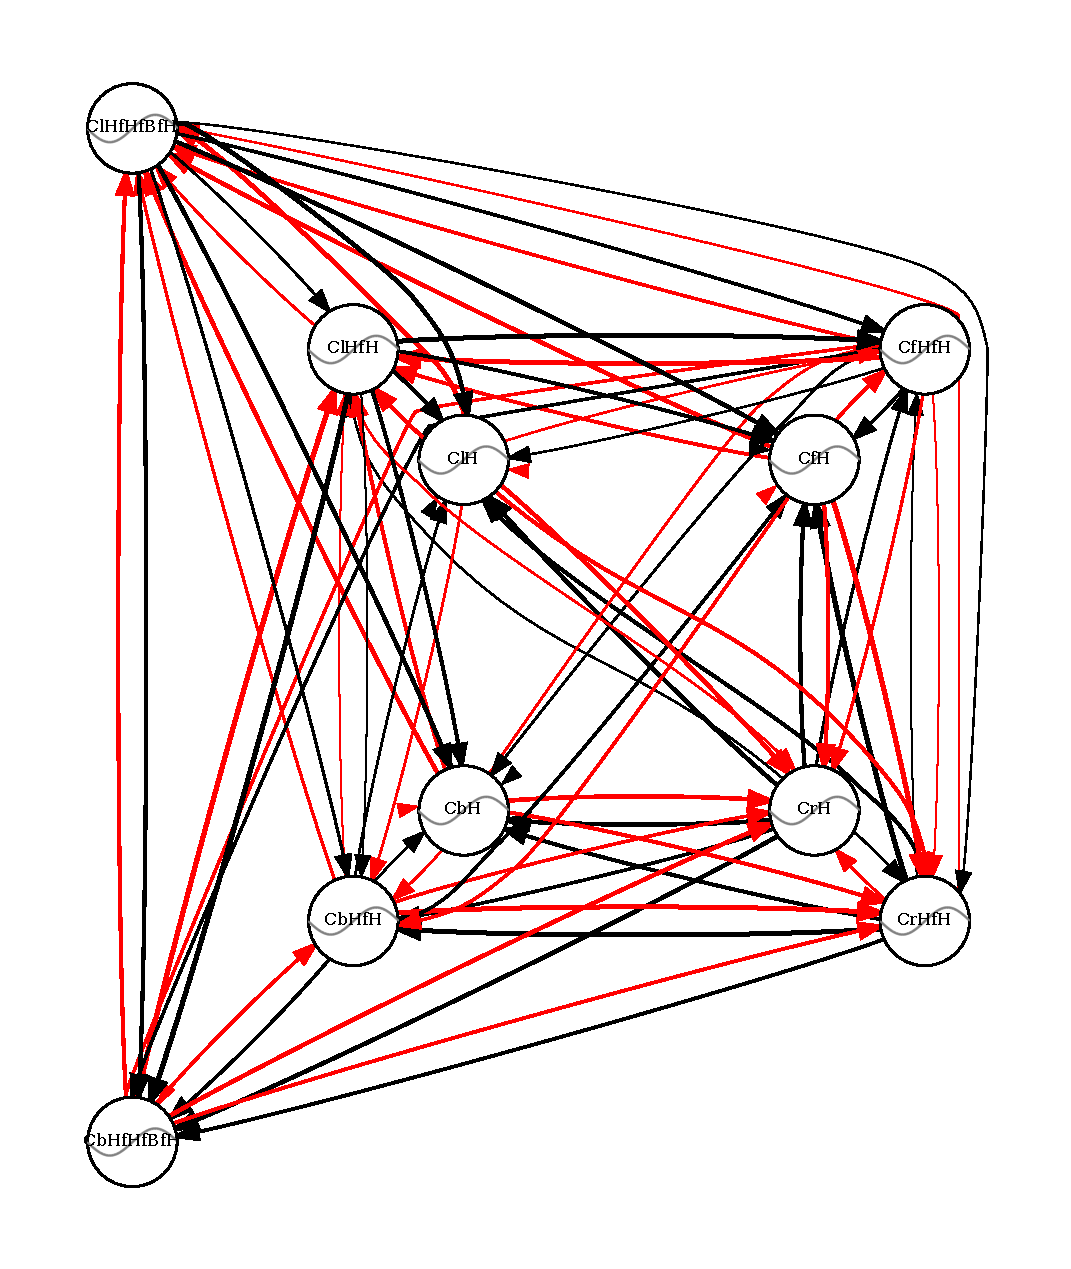
\includegraphics[width=1cm]{brain}};
 \node at (CPG_r) [fill=white, fill opacity=.5, text opacity=1] {CPG};

\ifnum\stage>1
 \node [above=.5cm of CPG_r] (abCPG) {$\alpha\beta-$CPG};
 \coordinate (policy_south) at ($(abCPG.north)+(0,.25)$);
 \node (abcpg_all) [fit=(CPG_r)(abCPG)(policy_south), draw] {};

 \draw [->] (CPG_r) -- (abCPG) node [pos=0.5, arrownode] {Raw control};
 \draw [->] (abcpg_all.north) -- (abCPG) node [pos=0.5, arrownode] {$\alpha,\beta$};

 \node (mc) [right=.5cm of abCPG, arrownode]
  {\begin{tabular}{@{}c@{}}Modulated\\control\end{tabular}};

 \draw (abCPG) -- (mc);
\fi
\ifnum\stage=2
 \draw [->] (mc) -- ++(1, 0);
\fi
\ifnum\stage>2
 \definecolor{ok0}{HTML}{0072B2}
 \definecolor{ok1}{HTML}{E69F00}
 \definecolor{ok2}{HTML}{009E73}
 \definecolor{ok3}{HTML}{CC79A7}
 \definecolor{ok4}{HTML}{D55E00}

 \foreach \i in {4,...,0} {
  \node [draw=ok\i, above=0cm of abcpg_all, shift={(-.1*\i,.1*\i)}, fill=black] (policy_\i) {Policy};
 }

 \foreach \i in {2,...,0} {
  \def\envs{{"fetch", "carrying", "obstacles"}}
  \node (env_\i) [draw=ok\i, ultra thick, above right=-.25cm and 2cm of abCPG, shift={(.1*\i,.1*\i)}, inner sep=0pt]
   {\pgfmathparse{\envs[\i]}\includegraphics[width=1.5cm]{../tasks/\pgfmathresult}};

%    \node [envnode, above=0 of env\i, fill=white, font=\small] (env_\i) {Simulation};

  \draw  [->, ok\i, thick] (env_\i) |- ++(0, 1.25) coordinate [pos=.5] (ed\i) -| (policy_\i.north);
 }
 \node [below=0 of env_0] {Simulation};

 \foreach \i in {4,3} {
  \node (env_\i) [draw=ok\i, ultra thick, below right=.75cm and 1.8cm of abCPG, shift={(.1*\i,-.1*\i)}, inner sep=0pt]
   {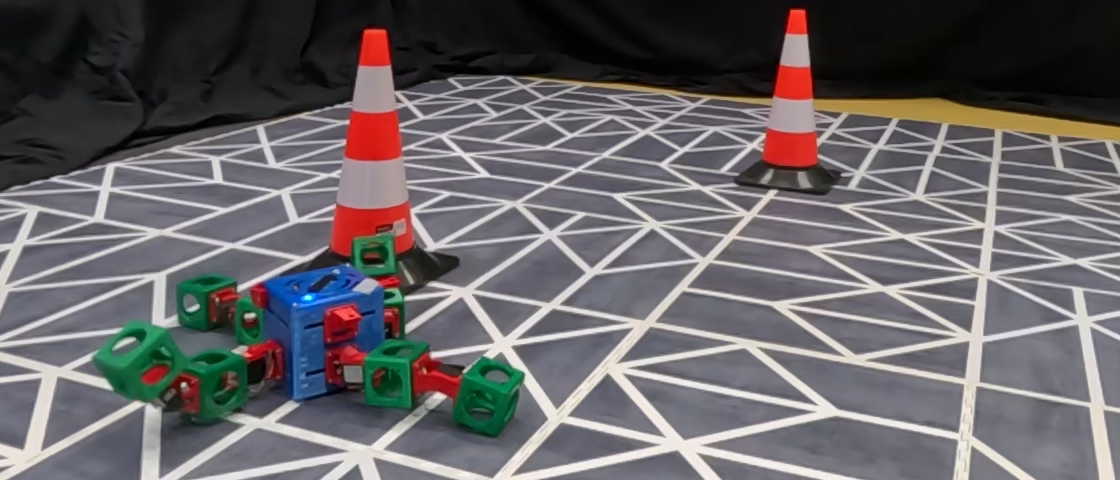
\includegraphics[width=1.5cm]{../hardware/slalom/t25}};
  \draw  [->, ok\i, thick] (env_\i.east) -| ++(.2, 3.45+.2*\i) -| (policy_\i.north);
 }
 \node [above=0 of env_3] {Real world};

 \draw [->] (mc) |- (env_3);
 \draw [->] (mc) |- (env_0);


 \node at (ed2-|mc) [arrownode, inner sep=1.5pt] {Observations};
\fi

\end{tikzpicture}}
\end{document}
